\chapter{Performance} \label{chap:performance}
This chapter discusses the performance of my system based on the implementation described in the previous chapter. The indicators used in the measurement includes but not limited to The response time and frequency of image collection.

The outcome is based on the physical devices used in the implementation. The measurement happens in the environment of the campus network. So the high-speed network is supported, and the end device(Nexus 6) accesses the Fog Nodes within one hop through a wireless access point.

The performance of the Fog Basic Mode is reported firstly. The response time and the frequency of requests are the variant parameters. This benchmark aims to narrow down the exact traffic of requests that Fog Nodes are capable of handling.

As we can see in the figure \ref{fig:response_time_fog_basic}, the response time fluctuate when the frequency of face detection is relatively high. On the contrary, the response time is stable when the frequency of images collection is between 1 image per second and 0.5 images per second.


\begin{figure}
\centering
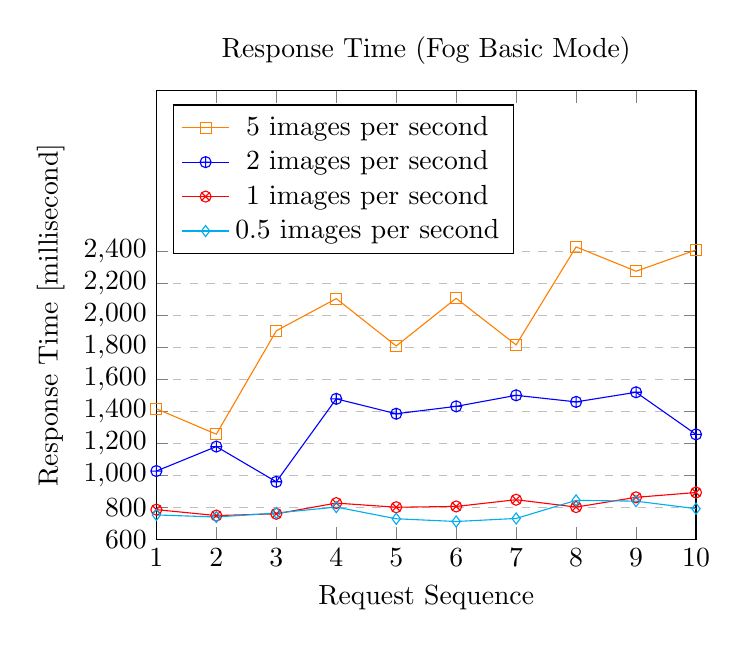
\begin{tikzpicture}
\begin{axis}[
    title={ Response Time (Fog Basic Mode)},
    xlabel={Request Sequence},
    ylabel={Response Time [millisecond]},
    xmin=1, xmax=10,
    ymin=600, ymax=3400,
    xtick={0,1,2,3,4,5,6,7,8,9,10},
    ytick={600, 800, 1000, 1200, 1400, 1600, 1800, 2000, 2200, 2400},
    legend pos=north west,
    ymajorgrids=true,
    grid style=dashed,
]
 
\addplot[
    color=orange,
    mark=square,
    ]
    coordinates {
    (1,1415)(2, 1256)(3,1902)(4,2103)(5, 1807)(6, 2105)(7, 1814)(8,2426)(9,2274)(10,2407)
    };
\addplot[
    color=blue,
    mark=oplus,
    ]
    coordinates {
    (1,1026)(2, 1179)(3,959)(4,1477)(5, 1384)(6, 1430)(7, 1499)(8,1458)(9,1518)(10,1255)
    };
 
\addplot[
    color=red,
    mark=otimes,
    ]
    coordinates {
    (1,785)(2, 748)(3,759)(4,826)(5, 800)(6, 805)(7, 847)(8,801)(9,862)(10,892)
    };
    
\addplot[
    color=cyan,
    mark=diamond,
    ]
    coordinates {
    (1,752)(2, 739)(3,764)(4,801)(5, 728)(6, 711)(7, 730)(8,843)(9,838)(10,791)
    };
    
\legend{5 images per second, 2 images per second, 1 images per second, 0.5 images per second}
\end{axis}
\end{tikzpicture}
\caption{Response Time (Fog Basic Mode)}
\label{fig:response_time_fog_basic}
\end{figure}

The statistics of the CPU usage is recorded to analyse the underlying cause of the fluctuation of the Response Time. In the figure \ref{fig:cpu_percentage_fog_basic}, the trend of CPU usage can be observed with the increasing traffic of images for face detection.

\begin{figure}
\centering
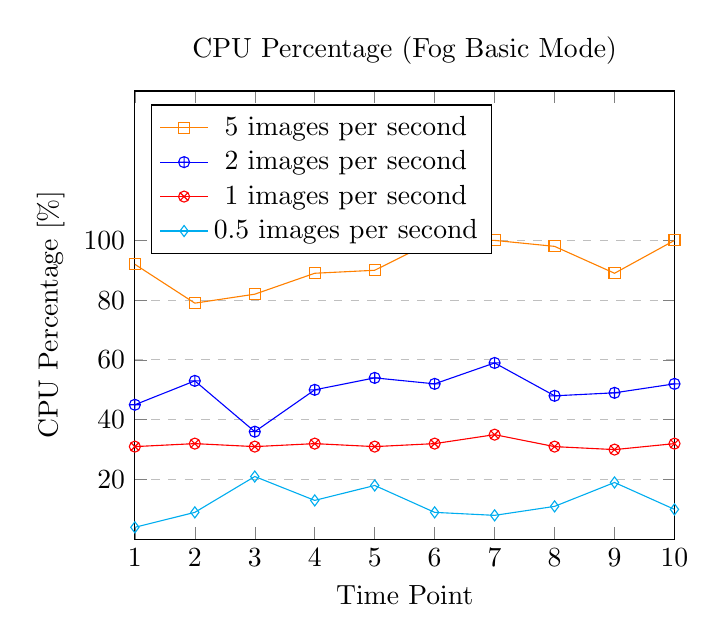
\begin{tikzpicture}
\begin{axis}[
    title={ CPU Percentage (Fog Basic Mode)},
    xlabel={Time Point},
    ylabel={CPU Percentage [\%]},
    xmin=1, xmax=10,
    ymin=0, ymax=150,
    xtick={0,1,2,3,4,5,6,7,8,9,10},
    ytick={ 20, 40, 60, 80, 100},
    legend pos=north west,
    ymajorgrids=true,
    grid style=dashed,
]
 
\addplot[
    color=orange,
    mark=square,
    ]
    coordinates {
    (1,92)(2, 79)(3,82)(4,89)(5, 90)(6, 100)(7, 100)(8,98)(9,89)(10,100)
    };
\addplot[
    color=blue,
    mark=oplus,
    ]
    coordinates {
    (1,45)(2, 53)(3,36)(4,50)(5, 54)(6, 52)(7, 59)(8,48)(9,49)(10,52)
    };
 
\addplot[
    color=red,
    mark=otimes,
    ]
    coordinates {
    (1,31)(2, 32)(3,31)(4,32)(5, 31)(6, 32)(7, 35)(8,31)(9,30)(10,32)
    };
    
\addplot[
    color=cyan,
    mark=diamond,
    ]
    coordinates {
    (1,4)(2, 9)(3,21)(4,13)(5, 18)(6, 9)(7, 8)(8,11)(9,19)(10,10)
    };
    
\legend{5 images per second, 2 images per second, 1 images per second, 0.5 images per second}
  

\end{axis}
\end{tikzpicture}

\caption{CPU Percentage (Fog Basic Mode)}
\label{fig:cpu_percentage_fog_basic}
\end{figure}


The figure \ref{fig:network_receiving_fog_basic} reveal the requirement of the precise network bandwidth. Even though campus network offers nearly unlimited bandwidth, comparing to the demand of this system, the realistic traffic deserves attention for a more confined environment in the future.

\begin{figure}
\centering
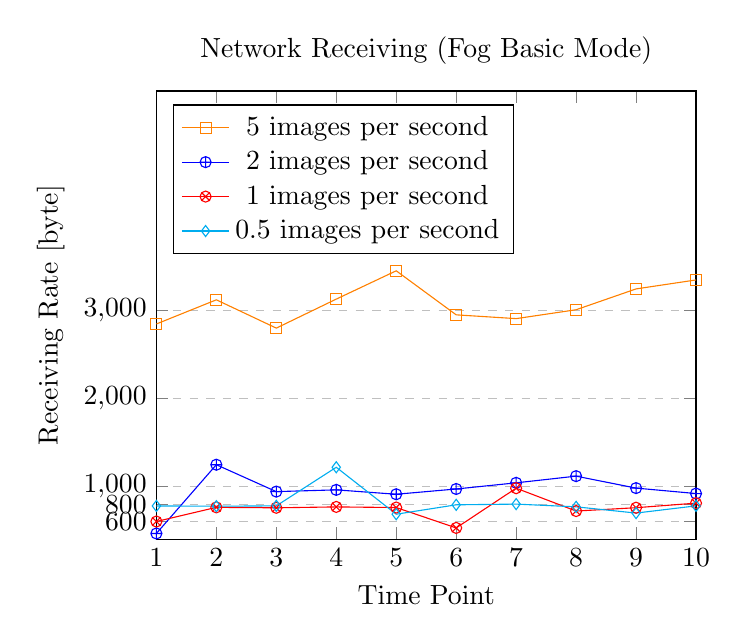
\begin{tikzpicture}
\begin{axis}[
    title={ Network Receiving (Fog Basic Mode)},
    xlabel={Time Point},
    ylabel={Receiving Rate [byte]},
    xmin=1, xmax=10,
    ymin=400, ymax=5500,
    xtick={0,1,2,3,4,5,6,7,8,9,10},
    ytick={ 600, 800, 1000, 2000, 3000},
    legend pos=north west,
    ymajorgrids=true,
    grid style=dashed,
]
 
\addplot[
    color=orange,
    mark=square,
    ]
    coordinates {
    (1,2849)(2, 3124)(3,2802)(4,3132)(5, 3454)(6, 2953)(7, 2910)(8,3011)(9,3248)(10,3350)
    };
\addplot[
    color=blue,
    mark=oplus,
    ]
    coordinates {
    (1,466)(2, 1248)(3,942)(4,962)(5, 912)(6, 972)(7, 1042)(8,1118)(9,982)(10,920)
    };
 
\addplot[
    color=red,
    mark=otimes,
    ]
    coordinates {
    (1,602)(2, 763)(3,758)(4,768)(5, 761)(6, 529)(7, 981)(8,721)(9,759)(10,811)
    };
    
\addplot[
    color=cyan,
    mark=diamond,
    ]
    coordinates {
    (1,779)(2, 776)(3,780)(4,1219)(5, 685)(6, 792)(7, 800)(8,769)(9,698)(10,780)
    };
    
\legend{5 images per second, 2 images per second, 1 images per second, 0.5 images per second}
  

\end{axis}
\end{tikzpicture}
\caption{Network Receiving on the Fog Node  (Fog Basic Mode)}
\label{fig:network_receiving_fog_basic}
\end{figure}

Table \ref{table:measure_response_time} shows the raw data sampled during the operation of the system. The data plotting line charts are generated by raw information in this format.

\begin{table}[h!]
\centering
\begin{tabular}{ |c|c|c| } 
 \hline
 send time-stamp &    receive time-stamp &    period\\
 \hline
14:55:18.741 &    14:55:19.767 &    00:00:01.026\\
14:55:19.249 &    14:55:20.428 &    00:00:01.179\\
14:55:19.944 &    14:55:20.903 &    00:00:00.959\\
14:55:20.309 &    14:55:21.786 &    00:00:01.477\\
14:55:20.820 &    14:55:22.204 &    00:00:01.384\\
14:55:21.285 &    14:55:22.715 &    00:00:01.430\\
14:55:21.747 &    14:55:23.246 &    00:00:01.499\\
14:55:22.301 &    14:55:23.759 &    00:00:01.458\\
14:55:22.795 &    14:55:24.313 &    00:00:01.518\\
14:55:23.316 &    14:55:24.571 &    00:00:01.255\\
14:55:23.829 &    14:55:25.306 &    00:00:01.477\\
14:55:24.234 &    14:55:25.979 &    00:00:01.745\\
14:55:24.779 &    14:55:26.167 &    00:00:01.388\\
14:55:25.266 &    14:55:27.080 &    00:00:01.814\\
14:55:25.834 &    14:55:27.278 &    00:00:01.444\\
14:55:26.408 &    14:55:28.150 &    00:00:01.742\\
14:55:26.816 &    14:55:28.338 &    00:00:01.522\\
14:55:27.461 &    14:55:29.175 &    00:00:01.714\\
14:55:27.912 &    14:55:29.662 &    00:00:01.750\\
14:55:28.343 &    14:55:30.112 &    00:00:01.769\\
 \hline
\end{tabular}
\caption{Sample of measuring Response Time (5 images per second)}
\label{table:measure_response_time}
\end{table}

The figure \ref{fig:response_time_fog_dnn} displays the outcome of the Fog DNN mode. Its measurement follows the same flow of sampling the response time of Fog Basic mode. Nevertheless, the gap is huge when it comes to the stable response time. From the chart, we can see the stable response time is about 5000 milliseconds. However, its counterpart in Fog Basic mode is just around 800 milliseconds. Also, the corresponding frequency is lower as well, approximately 0.2 images per second. Compared to the frequency of nearly 0.8 images per second, the delicate face recognition tasks drag the performance.

\begin{figure}
\centering
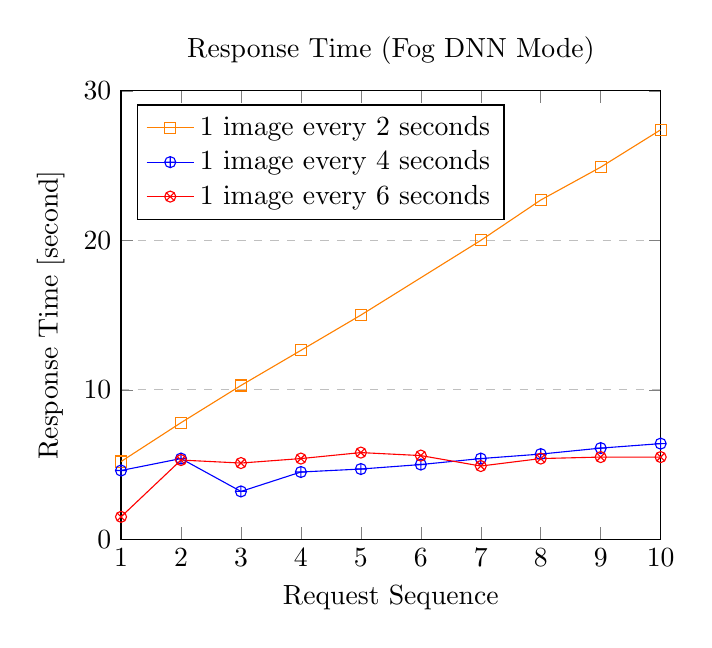
\begin{tikzpicture}
\begin{axis}[
    title={ Response Time (Fog DNN Mode)},
    xlabel={Request Sequence},
    ylabel={Response Time [second]},
    xmin=1, xmax=10,
    ymin=0, ymax=30,
    xtick={0,1,2,3,4,5,6,7,8,9,10},
    ytick={},
    legend pos=north west,
    ymajorgrids=true,
    grid style=dashed,
]
 
\addplot[
    color=orange,
    mark=square,
    ]
    coordinates {
    (1,5.2)(2, 7.8)(3,10.29)(4,12.64)(5, 15)(17.6)(7, 20)(8,22.7)(9,24.9)(10,27.4)
    };
\addplot[
    color=blue,
    mark=oplus,
    ]
    coordinates {
    (1,4.6)(2, 5.4)(3,3.2)(4,4.5)(5, 4.7)(6, 5)(7, 5.4)(8,5.7)(9,6.1)(10,6.4)
    };
 
\addplot[
    color=red,
    mark=otimes,
    ]
    coordinates {
    (1,1.5)(2, 5.3)(3,5.1)(4,5.4)(5, 5.8)(6, 5.6)(7, 4.9)(8,5.4)(9,5.5)(10,5.5)
    };
    
\legend{ 1 image every 2 seconds, 1 image every 4 seconds, 1 image every 6 seconds,}
  

\end{axis}
\end{tikzpicture}

\caption{Response Time (Fog DNN Mode)}
\label{fig:response_time_fog_dnn}
\end{figure}